%Document Class
\documentclass[12pt,letterpaper,oneside]{article}

%Packages
\usepackage{amsmath}
\usepackage[pdftex]{hyperref}
\usepackage[margin=1in]{geometry}
\usepackage{pdflscape}
\usepackage{setspace}
\usepackage{hyperref}
\usepackage{biblatex}
\bibliography{reference.bib}
\usepackage{listings}
\usepackage{MnSymbol}
\usepackage{tikz}
\usetikzlibrary{shapes,arrows}

%Settings
\setlength\parindent{0pt} %globally suppress indentation
\renewcommand{\rmdefault}{phv} % Arial
\renewcommand{\sfdefault}{phv} % Arial
\newcommand{\HRule}{\rule{\linewidth}{0.5mm}}
\graphicspath{{Images//}} %Path to pictures
\newcommand{\tab}{\hspace*{2em}} %Command for tab
\hypersetup{ %Sets up the hyperlinks in the TOC
colorlinks,
citecolor=black,
filecolor=black,
linkcolor=black,
urlcolor=black
}

\makeatletter
\lst@Key{numbers}{none}{%
\let\lst@PlaceNumber\@empty
    \lstKV@SwitchCases{#1}%
    {none&\\%
     left&\def\lst@PlaceNumber{\llap{\normalfont
                \lst@numberstyle{\thelstnumber}\kern\lst@numbersep}}\\%
     leftliteral&\def\lst@PlaceNumber{\llap{\normalfont
                \lst@numberstyle{\the\lst@lineno}\kern\lst@numbersep}}\\%
     right&\def\lst@PlaceNumber{\rlap{\normalfont
                \kern\linewidth \kern\lst@numbersep
                \lst@numberstyle{\thelstnumber}}}%
    }{\PackageError{Listings}{Numbers #1 unknown}\@ehc}}
\makeatother 

\makeatletter    
%\lst@UserCommand\lstlistlistingname{Code}
%\lst@UserCommand\lstlistingname{Code}

\def\lst@MProcessListing{%
    \lst@XPrintToken \lst@EOLUpdate \lsthk@InitVarsBOL
    \global\advance\lst@lineno\@ne
    \ifnum \lst@lineno>\lst@lastline
        \lst@ifdropinput \lst@LeaveMode \fi
        \ifx\lst@linerange\@empty
            \expandafter\expandafter\expandafter\lst@EndProcessListing
        \else
		\ifx\lst@OutputBox\@gobble\else
        \par\noindent \hbox{}%
    	\fi
          	{\bfseries\color{red} \ensuremath{\napprox}}
            \lst@interrange
            \lst@GetLineInterval
            \expandafter\expandafter\expandafter\lst@SkipToFirst
        \fi
    \else
        \expandafter\lst@BOLGobble
    \fi}
\makeatother
   
%Settings to properly display code in document
\lstloadlanguages{[GNU]C++, [x86masm]Assembler}
\lstset{%
tabsize=4,
numbers=leftliteral,
numberstyle=\tiny,
stepnumber=2,
numbersep=5pt,
basicstyle=\scriptsize\ttfamily,
breaklines=true,
escapeinside={\%*}{*)},
keywordstyle=\bfseries\color{green!40!black},
showstringspaces=false,
showspaces=false,
showtabs=false,
belowcaptionskip=6pt,
framexleftmargin=7mm,
frame=shadowbox,
rulesepcolor=\color{purple!60!black}
}
\lstset{prebreak=\raisebox{0ex}[0ex][0ex]
        {\ensuremath{\lcurvearrowdown}}}
\lstset{postbreak=\raisebox{0ex}[0ex][0ex]
        {\ensuremath{\rcurvearrowse\space}}}

\lstdefinestyle{customc}{
  breaklines=true,
  xleftmargin=\parindent,
  language=[GNU]C++,
  commentstyle=\itshape\color{purple!40!black},
  identifierstyle=\color{blue},
  stringstyle=\color{orange},
}

\begin{document}

\begin{titlepage}
\vspace*{\fill}
\begin{center}
	
%Title
{\huge \bfseries "Twisted" SIMON} \\[0.4cm]
Arduino Ignition Grant
\HRule \\[0.4cm]

% Authors/sponsors
\begin{minipage}{\textwidth}
\center
Zaza Soriano\\
Brian Taylor
\end{minipage}

\vspace*{\fill}

%Bottom of the page
{\large \today}
\end{center}
\end{titlepage}

\numberwithin{figure}{section} %Makes Figures numbered based on section
\numberwithin{table}{section}
\numberwithin{lstlisting}{section}
\pagenumbering{roman} %Page numbers roman before 1st section
\doublespace
\tableofcontents %Table of contentes
\newpage
%\listoffigures %Table of figures
%\newpage
%\listoftables %Table of tables
%\newpage
\lstlistoflistings %Table of listings
\newpage
\singlespace
\pagenumbering{arabic} %Page numbers normal from now on
			
\section{Goals}
To learn about various sensors and how they interact with the Arduino by making a game based off of the classic game of SIMON.

\section{References} \label{sec:ref}
\url{http://www.instructables.com/id/Arduino-Simon-Says}\\
\url{http://www.instructables.com/id/Stickytape-Sensors/step5/Velostat}

\section{Hardware}
		\begin{itemize} \parskip0pt
			\item Arduino Board
			\item USB Cable
			\item Breadboard
			\item Wires
			\item 5 x Resistor 220$\Omega$
			\item 4 x LED
			\item 4 x Button
			\item Speaker
			\item Rotary Knob (Potentiometer)
			\item Light Sensor (Photocell)
			\item Motion Sensor (Tilt Switch)
			\item Temperature Sensor
			\item Conductive Fabric
			\item Conductive Thread
			\item Velostat
			\item Tape
			\item Scissors
		\end{itemize}

\section{Discussion}

	\subsection{SIMON} \label{sec:simon}
"Think fast... SIMON, 'Chase my flashing lights and sounds'!"\bigskip
\\The classic SIMON is a computer-controlled game that consists of a base unit with 4 color lenses and a control panel. The challenge is to repeat the ever-increasing random signals that SIMON generates. If the pattern you respond is correct SIMON will add another light to the pattern.\bigskip
\\"Twisted" Simon is a game that is controlled by an Arduino. It will have 4 LEDs each with it's own way to activate it. The LEDs could be activated by the press of a button or a flashlight, just to name a few examples (as the options are endless). The Arduino will start by lighting up a random LED, at witch point the Player will activate the appropriate LED in response (hint: the correct LED is the one the Arduino lit up). If correct, the Arduino will add a random LED to the sequence (which is now 2 long) and the process repeats itself. If the Player enters the wrong sequence, the game is lost and the Player must start over.

	\subsection{Wiring the Arduino} \label{sec:wire}
	
	
	\subsection{Making a Push Sensor}
		\begin{enumerate}
				\item Gather your materials
					\begin{enumerate}
						\item 3 pieces of velostat (same size)
						\item 2 pieces of tape (slightly larger than the velostat)
						\item 2 strands of conductive thread (about the length of the velostat)
						\item 2 pieces of conductive fabric (enough for the alligator clip to work with)
					\end{enumerate}
				\item Place a conductive thread and fabric onto the sticky side of a piece of tape, show in Figure \ref{fig:stickyTape}
					\begin{figure} [here]
						\centering
						\caption{Push sensor insides}
						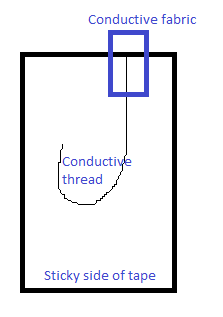
\includegraphics[scale=.6]{sensor.png}		
						\label{fig:stickyTape}
					\end{figure}	
				\item Repeat previous step
				\item Sandwich velostat between tape making sure to overlap the conductive thread
		\end{enumerate}						

\section{Procedure}
		
		\subsection{"Not so twisted" SIMON}
			\begin{enumerate}
				\item Wire the Arduino with 4 LED's, 4 push buttons, and 1 speaker (See Section \ref{sec:wire})
				\item Load the Twisted\_Simon\_Says.ino file onto the Arduino (See Appendix \ref{lst:twistedSimon})
			\end{enumerate}
								
		\subsection{"Twisted" SIMON}
			\begin{enumerate}
				\item Replace one of the push buttons with an analog sensor
				\item Change the appropriate sensor information in the code, as an example look at line 21 in Listing \ref{lst:analog1}.
					\begin{center}
						\begin{minipage}{.9\textwidth}
							\lstinputlisting[caption={Twisted SIMON Sensors}, label=lst:analog1, style=customC, linerange={7-21}]{Code/Twisted_Simon_Says.ino}
						\end{minipage}
					\end{center}
					To get correct threshold value, uncomment the debug lines (shown in Listing \ref{lst:analog2}), run the program, and use the serial monitor to pick an appropriate threshold for the analog sensor. 
					\begin{center}
						\begin{minipage}{.9\textwidth}
							\lstinputlisting[caption={Twisted SIMON Debug}, label=lst:analog2, style=customC, linerange={49-56,147-151}]{Code/Twisted_Simon_Says.ino}
						\end{minipage}
					\end{center}
				\item Load the modified Twisted\_Simon\_Says.ino file onto the Arduino
			\end{enumerate}
			\newpage
			
		\subsection{Future SIMON}
			
\appendix
\section{\\Arduino Code} \label{App:AppendixA}
	\begin{center}
		\lstinputlisting[caption={Twisted SIMON Code}, label=lst:twistedSimon, style=customC]{Code/Twisted_Simon_Says_2.ino}	
	\end{center}	
\newpage		
\printbibliography

\end{document}
